%!TEX root = ../main.tex
\chapter{IL-RBMの強化学習への応用}\label{ch:ilrbm}
この章では,IL-RBMを本システムにおける強化学習への応用について説明する.


\section{強化学習}
強化学習\cite{RL木村}とは,あるエージェントがある環境内にて,得られる報酬を最大化するような行動を学習するような機械学習のことである.

図\ref{fig:el}に示すように,強化学習には重要な4つの概念があり,それらが相互作用を行う.

\begin{figure}[tb]
 \begin{center}
  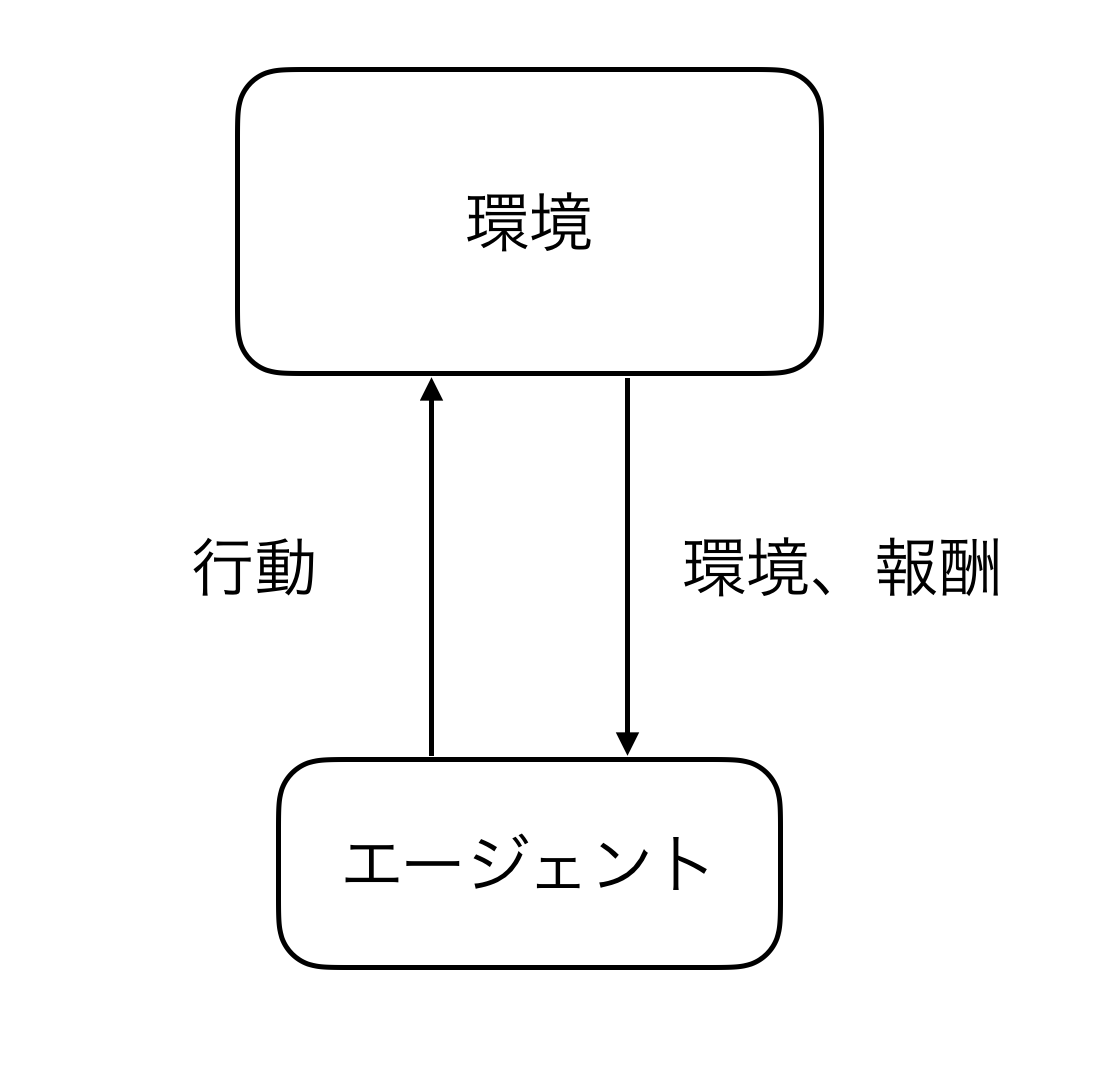
\includegraphics[scale=0.4]{./koki/el.png}
  \caption{強化学習の概要}
  % \ecaption{Representations of Data} 
  \label{fig:el}
 \end{center}
\end{figure}


\begin{itemize}
  \item 環境 … エージェントの行動に応じて,報酬をエージェントに与える.また,エージェントの行動に応じて,エージェントの観測する環境も更新される.
  \item 報酬 … エージェントの行動に応じて環境からエージェントに与えられる.この得られる報酬を最大化するようエージェントは行動を学習する.
  \item 行動  … エージェントは観測した環境に応じて,行動を選択する.
  \item エージェント … 環境を観測し,報酬を受け取り,行動を選択する.
\end{itemize}

明確な教師データが与えられる教師あり学習や,全く教師データが与えられない教師なし学習と異なり,報酬という限定されたフィードバックのみが与えられる点に特徴がある.
不確実な環境を取り扱えるという点で,応用上非常に有望な機械学習手法の一つである.

また,強化学習とニューラルネットワークを併用する研究も盛んであり,この分野で近年非常に有名になった研究に,ディープニューラルネットワークと強化学習の一手法であるQ学習\cite{watkins1992q}を組み合わせたDeep Q Networkと呼ばれる手法を提案し,それを用いてビデオゲームを解かせたものがある\cite{mnih2013playing}.

また,私達人間の脳内においても環境から与えられる報酬を予測していることが示唆されており\cite{schultz1997neural},上述した強化学習に近いメカニズムを脳内に持っていると予想されている\cite{銅谷}.
また,計算論神経科学の分野でも強化学習を人類の脳と関連付ける研究が盛んに行われている\cite{lee2012neural,izhikevich2007solving,maia2011reinforcement}.



\section{エージェントの概要}
エージェントの概要について具体的に説明する.

図\ref{fig:ildbn}に示す通り,本システムで用いたエージェントは,IL-RBMと出力層からなるDBN(以下,IL-DBN)を用いている.出力層はパーセプトロンで構成されている.このIL-DBNは入力データを環境,出力を行動として学習する.

\begin{figure}[tb]
 \begin{center}
  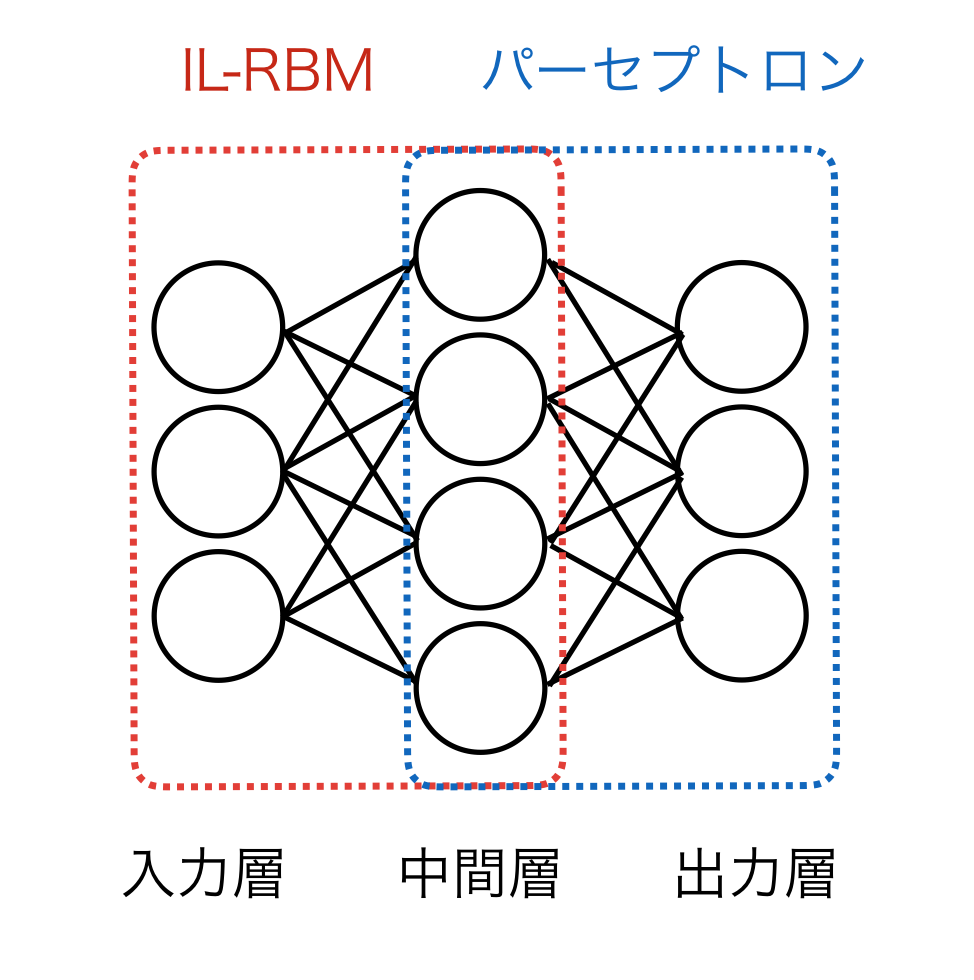
\includegraphics[scale=0.6]{./koki/ildbn.png}
  \caption{IL-DBN}
  % \ecaption{Representations of Data} 
  \label{fig:ildbn}
 \end{center}
\end{figure}


エージェントは,常に今自分が置かれている環境を観測することが可能であり,環境から報酬を与えられた場合には,それを感知することが可能である.

エージェントは環境と行動の組からなるデータセットを自動的に構築し,そのデータセットを逐次的に学習することで,最適行動を学習する.
また,IL-RBMのエネルギーに注目することで,未学習データセットを検出できるという特徴を用い,後述するサブゴールを獲得し,長期的な戦略を獲得することが可能である.どのようにデータセットを収集するかについての具体的手法について,次節から述べる.

\section{未学習データ判定法}

以下,文献\cite{osawa}内にて提案されている,未学習データ判別法について述べる.\ref{sec:learn}で説明したとおり,RBMは以下に$J$で表される対数尤度を最大化するように学習が行われる.すなわち,エネルギー$E$を最小化するように学習が行われることと同値である.

\begin{eqnarray}
	p(\bm{v}, \bm{h}; \theta) & = & \frac{1}{Z(\theta)}  \exp (-E(\bm{v},\bm{h};\theta)) \nonumber \\
	E(\bm{v}, \bm{h}; \theta) & = & -\sum_i b_i v_i - \sum_j c_j h_j- \sum_i \sum_j v_i W_{ij} h_j \nonumber \\
	p(\bm{v};\theta) & = & \sum_{\bm{h}} p(\bm{v},\bm{h};\theta) \nonumber \\
			& = & \sum_{\bm{h}} \frac{1}{Z(\theta)} \exp (-E(\bm{v}, \bm{h}; \theta)) \nonumber \\
	J & = & < \ln \sum_{\bm{h}} p(\bm{v}, \bm{h}; \theta) >_q \nonumber \\
	  & = & < \ln \sum_{\bm{h}} \exp (-E(\bm{v}, \bm{h}; \theta) >_q - \ln Z(\theta) \nonumber 
\end{eqnarray}

したがって,学習済みRBMは既学習データが入力された場合はエネルギーが低くなり,未学習データが入力された場合にはエネルギーが高くなる.この原理を応用し,あるデータが入力された際のRBMのエネルギーを判定することで未学習データか既学習データかの判定を行う.

未学習データを入力した際のエネルギーと既学習データを入力した際のエネルギーをそれぞれ記録しておき,この値に基づいてある閾値を決定し,未学習か既学習か不明であるデータが入力された際のRBMのエネルギーが,この閾値を上回れば未学習,下回れば既学習と判定する.

\section{データセットの獲得}

本システムがデータセットを環境中から自動で学習するメカニズムについて説明する.
以下,三目並べタスクの最適行動を学習するエージェントを例に説明する.

学習エージェントが対戦相手と三目並べを行う環境下で,三目並べに勝利した場合と敗北した場合にそれぞれ正の報酬と負の報酬を与えられるとする.この時,エージェントが観測する環境は盤面の状態であり,出力する行動は次に選択する手の盤面上の位置となる.

\subsection{勝利データセットの獲得}
まず,エージェントは勝利データセットを収集する.ある行動を出力した際,盤面が勝利条件を満たし,正の報酬が与えられたとする.その勝利条件を満たした際の行動と,その行動をとった際の環境を組みにしてデータセットとしてエージェントは保存する.

\begin{figure}[tb]
 \begin{center}
  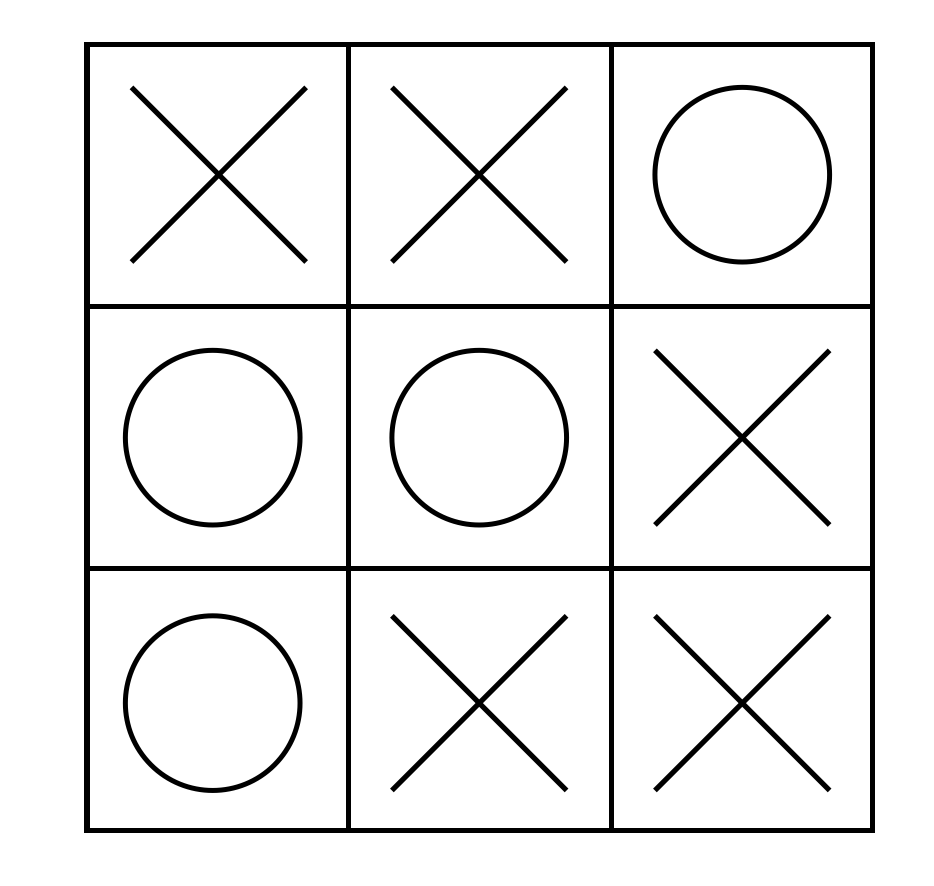
\includegraphics[scale=0.4]{./koki/ds.png}
 % ○が後攻,学習エージェント,
  %×が先行,相手エージェントを表す.
   \caption{勝利データセット例}
  % \ecaption{Representations of Data} 
  \label{fig:ds}
 \end{center}
\end{figure}

データセットがある一定数に達した場合,または試行回数が一定数に達した場合,エージェントは保存したデータセットを用いて学習を行う.

\subsection{サブゴールの獲得}
前述した,既学習,未学習判定を用いてサブゴールを獲得し,長期的な戦略を獲得するメカニズムについて説明する.

勝利データセットの獲得において,盤面が勝利条件を満たした場合,その時にとった行動と,行動を選択した際の環境を組みにしてデータセットとして保存した.
この場合,勝利条件を満たした盤面の状態をゴールとしてデータセットを採集している.

サブゴールとは,ゴールにつながり得る環境の状態を指す.
サブゴールを適切に設定し,サブゴールに至る行動と,その行動を選択した際の環境を更にデータセットに加える事で,長期的な戦略を獲得することができる.

\begin{figure}[tb]
 \begin{center}
  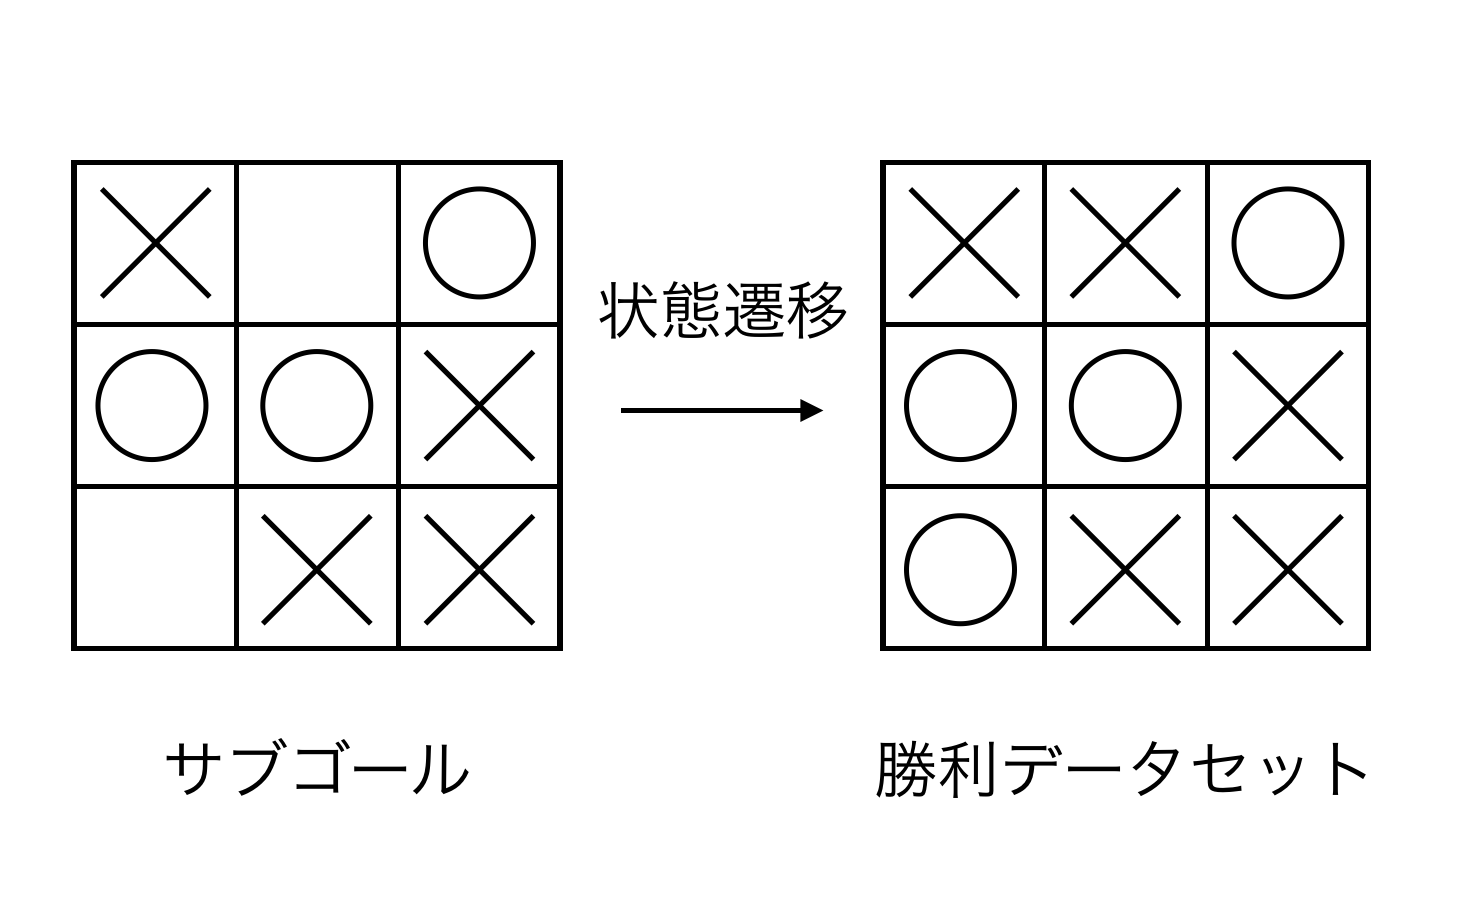
\includegraphics[scale=0.4]{./koki/sg.png}
   \caption{サブゴールの設定}
  % \ecaption{Representations of Data} 
  \label{fig:sg}
 \end{center}
\end{figure}


サブゴールの設定方法について説明する.ある行動を選択し,環境が更新されたとする.
その際の環境をエージェントのRBMが既学習であるか未学習であるかを前述したエネルギーによる判定法で判定する.
そして,得られた環境が既学習であった場合,その環境はゴールへと至る可能性が高いため,その環境をサブゴールとして設定する.
そして,サブゴールに至る直前の環境と,その状態にて選択した行動をデータセットとして新たに保存し,追加学習を行う.

\begin{figure}[tb]
 \begin{center}
  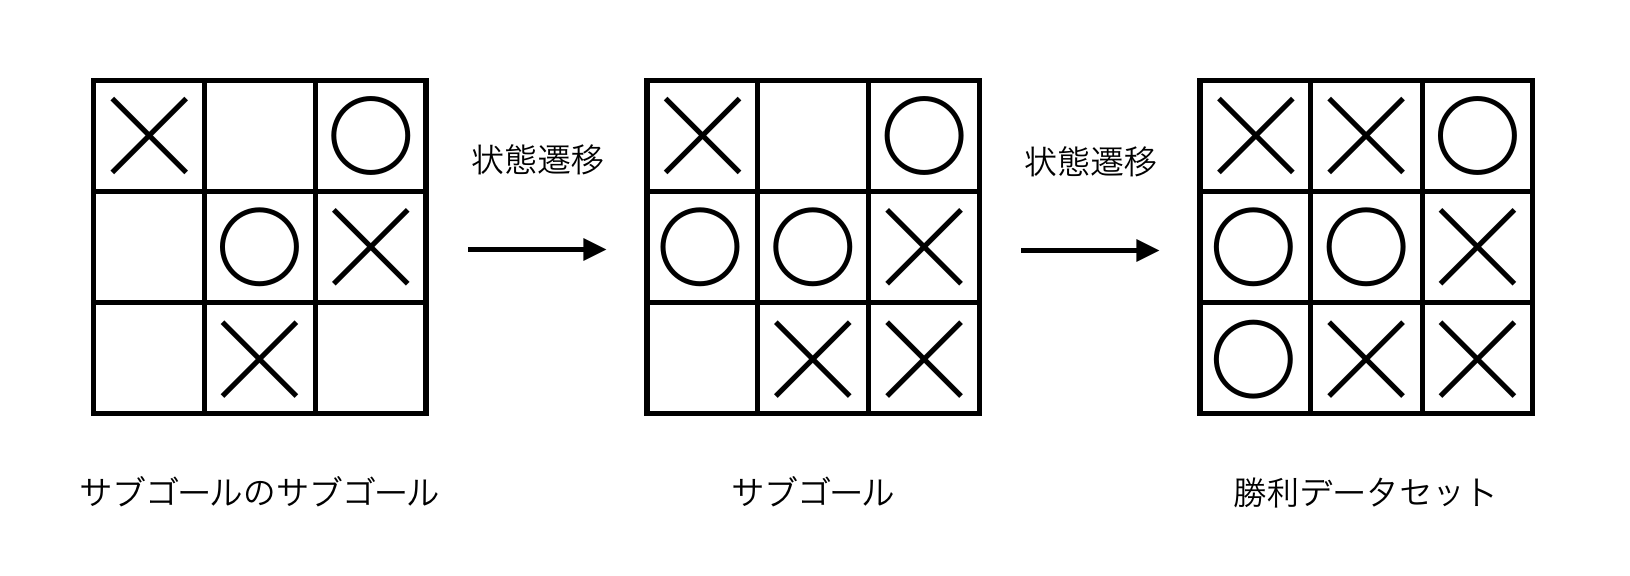
\includegraphics[scale=0.5]{./koki/sgsg.png}
   \caption{サブゴールのサブゴールの設定}
  % \ecaption{Representations of Data} 
  \label{fig:sgsg}
 \end{center}
\end{figure}


このようにして,図\ref{fig:sgsg}に示したとおり,サブゴールについても学習したIL-RBMは,また新たに'サブゴールのサブゴール'を扱うことが可能になる.観測された環境が,既に学習済みであるサブゴールである環境と一致,近似すると判定された場合,さらにその環境に至る行動とその直前の環境をデータセットとして加えることで,サブゴールのサブゴールを学習でき,長期的な戦略を獲得することが可能である.

\section{負のネットワーク,負のサブゴール}
前述したサブゴールの設定法には負の報酬と行動の抑制を扱えない,という欠点があった.
あるRBMがある環境を表す入力データを未学習か既学習か判定できたとしても,その環境が正の報酬に紐付いているか,負の報酬に紐付いているかを判定できないからである.

そこで,図\ref{fig:hn}に示すように負の報酬と負の報酬を得る環境へ至る行動を抑制するために負の報酬をあつかうネットワークをエージェントに追加することにした.

\begin{figure}[tb]
 \begin{center}
  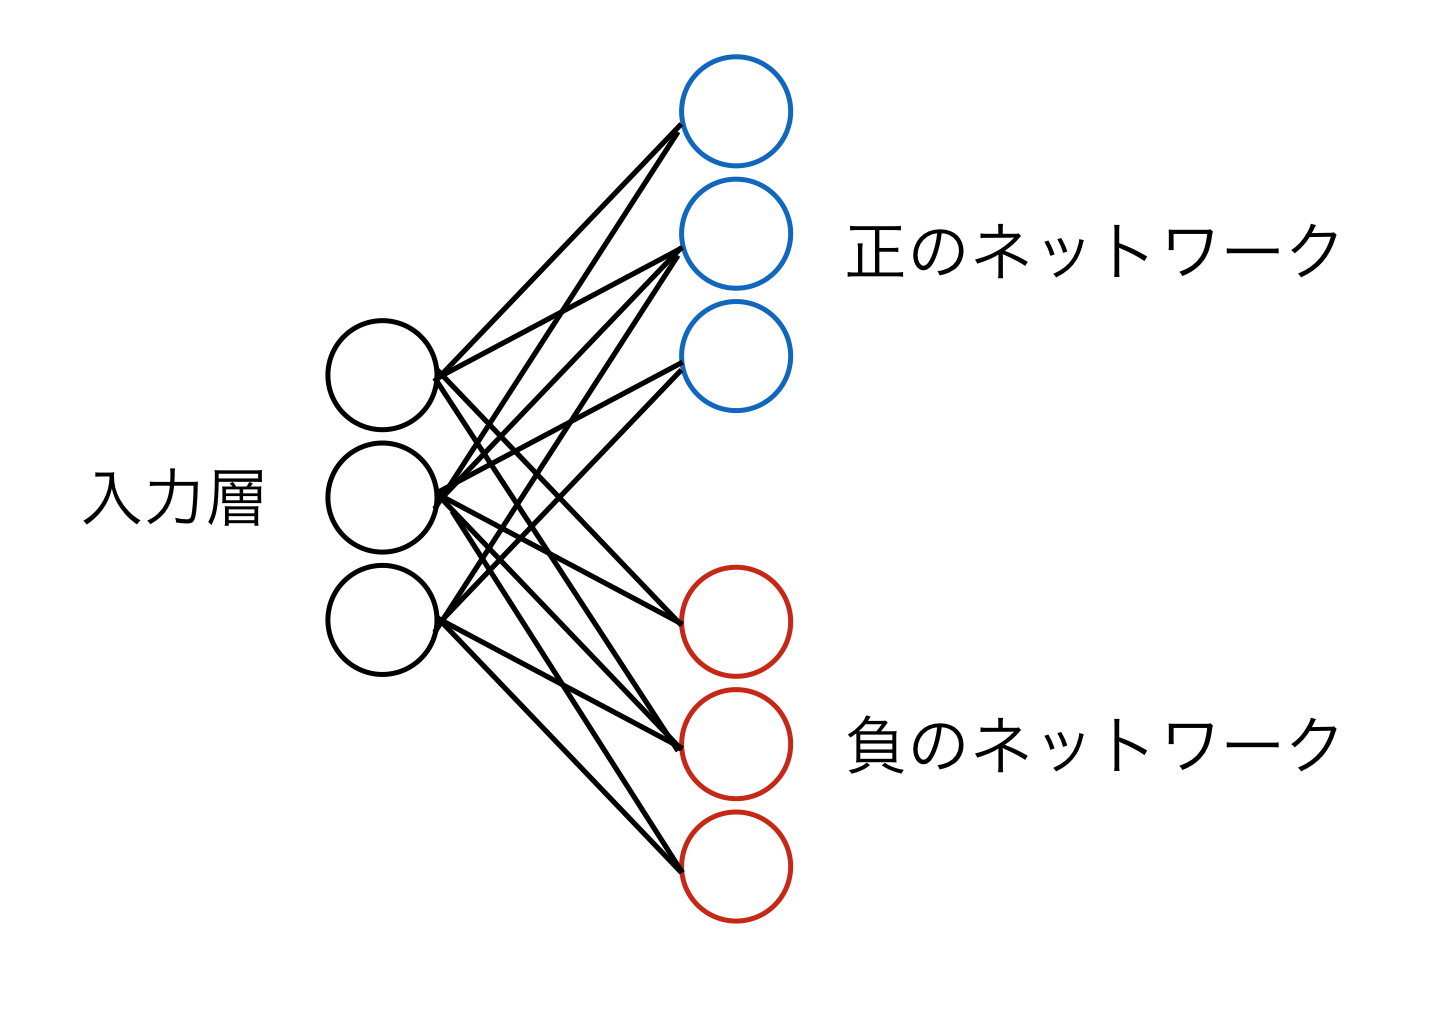
\includegraphics[scale=0.4]{./koki/hn.png}
  \caption{負のネットワーク}
  % \ecaption{Representations of Data} 
  \label{fig:hn}
 \end{center}
\end{figure}

エージェントはIL-RBMを二つ使用する.それぞれ正の報酬を扱うネットワークと負の報酬を扱うネットワークである.
また,保持するデータセットも二種類用意する.正の報酬を得ることのできるゴールに至る行動と,その直前の環境の組,サブゴールに至る行動とその直前の環境の組をデータセットとして扱う正のデータセットと,負の報酬について同様に扱う負のデータセットである.

負のデータセットを扱う負のネットワークでは,負の報酬を得ることになるゴール,サブゴールに至る行動が出力され,その直前の環境が入力データとなる.したがって,観測された環境をこのネットワークに入力した際の出力された行動は抑制されるべき行動である.

本エージェントでは負のネットワークからの出力を正のネットワークからの出力から引くことで,負の報酬を得る環境へ至る行動を抑制している.
%しかし,正のネットワークと負のネットワークを同列に扱うべきか,荷重をかけどちらかを優先すべきかなどは研究途中である.

\section{三目並べシステムの概要}

本システムは,強化学習の基本的な考え方に則り,'環境'と'エージェント'が'行動'と'報酬'により相互に影響を及ぼし合うように構成されている.

システムの流れは以下のとおりである.

\begin{enumerate}
  \item 二つのエージェントを定義する.
  \item 先行のエージェントに盤面の状態を与える.
  \item 先行のエージェントは盤面の状態から行動を選択する.
  \item 環境は,エージェントの行動を受け取り,自身の状態を更新する.
  \item 環境の状態に応じて,エージェントに報酬を与える.
  \item 環境の状態が終了条件を満たせばゲームを終了する.
  \item 上記手順を先攻,後攻を交代し繰り返す.
\end{enumerate}



環境部分は,常にある状態をを持ち,その状態はエージェントの行動によって変化させられる.また,環境部はその状態とエージェントの行動によってエージェントに与える報酬を決定する.

本システムは強化学習の基本的な考え方に則り,環境とエージェントの相互作用を取り扱う.

\subsection{環境部}
環境部はエージェントと環境の相互作用を制御するmainオブジェクトと,三目並べタスクの詳細の動作,情報を制御するThreePieceオブジェクトからなる.

\subsubsection{mainオブジェクト}
mainオブジェクトは,プログラム全体の制御を行う.

まず,行うタスクを定義する.今回行うタスクは三目並べであるためThreePieceオブジェクトをタスクとして定義する.その後,タスクの要請する数のエージェントを定義する.今回の実験では,先行のエージェントをランダムエージェント,後攻のエージェントをIL-DBNエージェントとした.

その他,エージェントと環境の相互作用を制御し,三目並べの終了時にThreePieceオブジェクトとエージェントのリセットを行ったり,三目並べを何ターン行うかの制御,それぞれのエージェント数の勝利数の保持を行う.

\subsubsection{ThreePieceオブジェクト}
ThreePieceオブジェクトは三目並べタスクを実際に執り行う.
ThreePieceオブジェクトはターン制でそれぞれのエージェントに盤面の情報を渡し,行動情報を受け取る.
盤面の情報の次元数や行動情報の形式はThreePieceオブジェクトが決定し,エージェントがアーキテクチャをその形式に合わせる.

盤面の情報はそれぞれのマスに対し,空白ならば(0,0),白石が置かれていれば(0,1),黒石が置かれていれば(1,0)の2bitで表現する.したがって9マス全体の表現は18次元の(0,0,0,1,1,0,0,0,0,1,0,0,0,0,0,0,1,0)のような表現になる.

一方エージェントの行動は0〜8の整数値で表される.それぞれの数値が石を置く盤面上の位置を示している.

%一方,エージェントの行動は9次元のベクトルで表現される.配置する石の位置に対応する次元の値のみ1で,それ以外は0のベクトルで表す.

ThreePieceオブジェクトはエージェントから渡された石の置き位置を示す値がルール上正当なものかを判定する.エージェントが石を置こうとしている場所に既に石が置かれている場合はエージェントに再度行動を選択するように命令する.指定された石の置き位置が正当であれば,オブジェクトの保持する盤面の状態を更新する.

その後,盤面の状態が三目並べの終了条件を満たしているかを判定する.盤面の状態を監視し,縦,横,斜めいずれかの方向に石が3つ並んでいれば,勝利エージェントへ報酬1を,敗北エージェントへ報酬-1を与える.

\subsection{エージェント部}
エージェントは基本的なエージェントの振る舞いを規定するAgentクラスがあり,それを継承することでそれぞれのAgentのクラスが作られている.

エージェントは環境から盤面状態を受け取った後,行動選択を行う.ランダムエージェントであれば0〜8で乱数を返し,学習エージェントは学習した行動を出力する.

環境が行動を受け取った後,エージェントは環境から報酬を受け取る.学習エージェントは報酬に応じて学習を行う.その学習の具体的なプロセスについては後述する.

\subsubsection{学習エージェント}
学習エージェントは次のような流れで学習を行う.


\begin{enumerate}
  \item 環境から状態が与えられる.
  \item 環境が記憶済みの状態の場合,一つ手前の状態とその状態でとった行動をデータセットに追加する.
  \item 行動選択後,環境から報酬が与えられる.
  \item 報酬に応じて状態と行動の組をデータセットに追加する.
  \item 上記の1から4を一定回数繰り返す.
  \item 採集したデータセット用いて追加するRBMのノード数を決定する.
  \item ノード数の確定したRBMを採集したデータセットで学習させる.
  \item データセットを空にリセットし1から再度データセットを採集する.
\end{enumerate}

学習エージェントには,負のネットワークを実装したものとしていないものの二種類あり,それらの勝率,敗北率を実験にて比較する.


